\documentclass{beamer}
\usetheme{Luebeck}
%\usetheme{Warsaw}
%\usetheme{Singapore}
\usecolortheme{lily}
%mode<presentation> {
%  \usetheme{Luebeck}
%  \usecolortheme{lily}
%  \beamertemplatenavigationsymbolsempty
%  \setbeamertemplate{headline}{}
%}
\usepackage{lmodern}
%\usepackage[affil-it]{authblk}


% include necessary packages here
\usepackage{graphicx} % for including images
\graphicspath{ {./png/} } % declare the path where your graphic files are
\DeclareGraphicsExtensions{.png} % so you won't have to specify these with every instance of \includegraphics
\usepackage{pgf} % for logo

\title{DCP and impact of exchange rates on trade}
\author{Nino Kodua and Tung-Sheng Hsieh}
\institute{Johns Hopkins University}
\date{April 6 2021}

\begin{document}
\maketitle

\section{Introduction}
\section{Impact of dominant currency on trade}
\subsection{Trade Volume Elasticity}
\begin{frame}{Trade Volume Elasticity}
    \begin{itemize}
        \item The paper has shown the stable bilateral terms-of-trade and an outsized effect of the dollar on trade prices.
        \item Now we explore if the country-level data is aligned with the model's implications on dollar's effect on trade volume. 
    \end{itemize}
\end{frame}
\begin{frame}{Trade Volume Elasticity}
    \begin{itemize}
            \item \emph{For non-US countries, import quantities should be driven by the dollar exchange rate as opposed to the bilateral exchange rate. }
            \item \emph{US import quantities should be less responsive to dollar exchange rate movements as compared to non-US countries.}
        \end{itemize}
\end{frame}
\begin{frame}{Trade Volume Elasticity}
\begin{itemize}
    \item Panel regression function
    \begin{equation*}
        \begin{aligned}
            \Delta y_{i j, t}= &\lambda_{i j}+\delta_{t}+\sum_{k=0}^{2} \beta_{k} \Delta e_{i j, t-k}+\sum_{k=0}^{2} \beta_{k}^{\$} \Delta e_{\$ j, t-k}\\
            &+\sum^{2}_{k=0} \eta_{k} \Delta e_{i j, t-k} \times S_{j}+\sum^{2}_{k=0} \eta_{k}^{\$} \Delta e_{\$ j, t-k} \times S_{j}+\theta^{\prime} X_{j, t}+\varepsilon_{i j, t}
        \end{aligned}
    \end{equation*}
    \item $\Delta y_{ij,t}$ denotes the log volume of goods exported from country $i$ to country $j$. $\Delta e_{i j, t-k}$ is the change in the (log) bilateral exchange rate between country $i$ and country $j$ at time $t-k$, expressed as the price of currency $i$ in terms of currency $j$; $S_j$ is the importing country's dollar invoicing share.
    \item $\lambda_{ij}$ and $\delta_t$ are dydadic and time fixed effects; $X_{j,t}$ consist of the log growth rate of real GDP (and two lags) for the importing country $j$.
\end{itemize}
\end{frame}
\begin{frame}{Trade Volume Elasticity}
    \begin{figure}[htp]
        \centering
        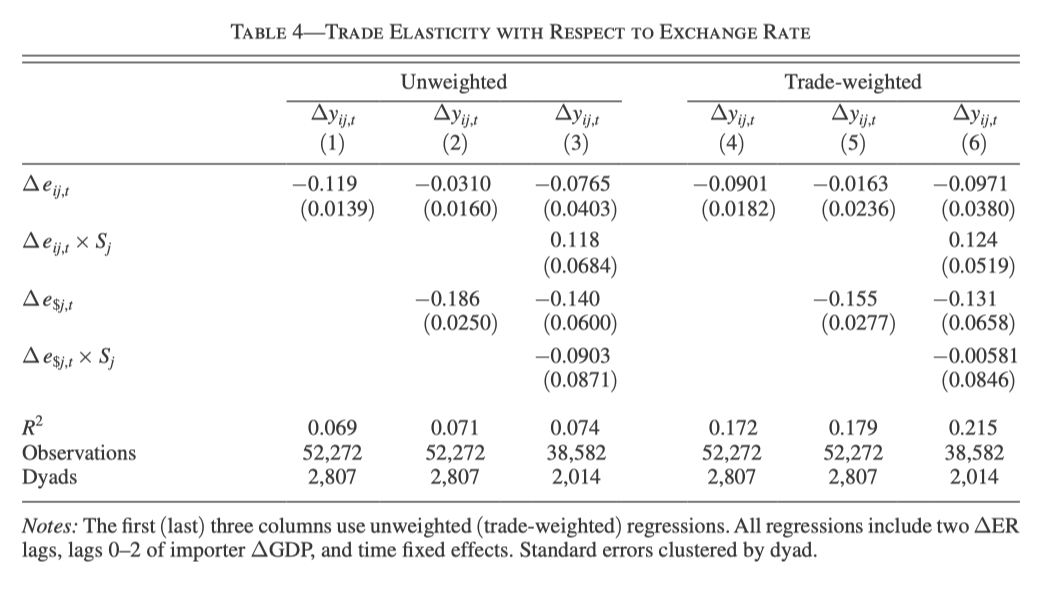
\includegraphics[width=11cm]{Table4.png}
    \end{figure}
\end{frame}
\begin{frame}{Trade Volume Elasticity}
    \begin{figure}[htp]
        \centering
        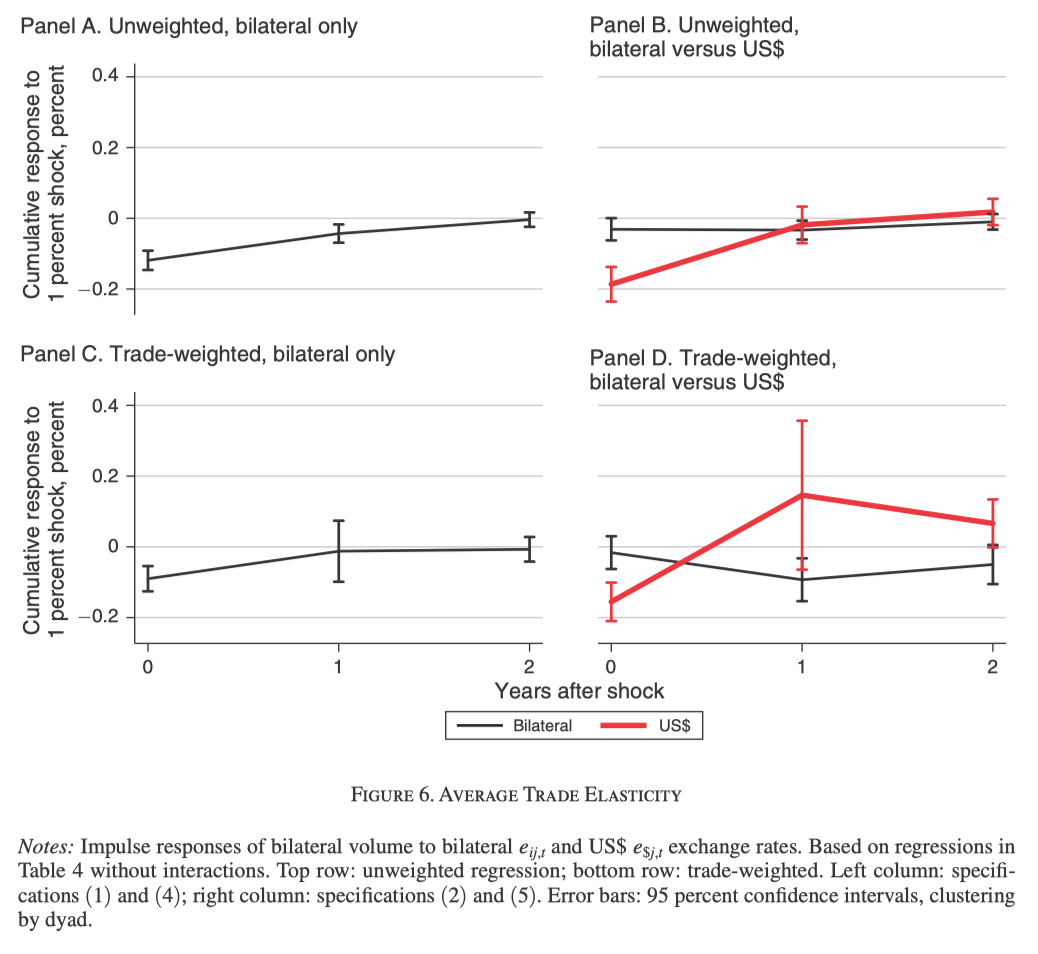
\includegraphics[width=8cm]{Figure6.png}
    \end{figure}
\end{frame}
\begin{frame}{Trade Volume Elasticity}
    \begin{figure}[htp]
        \centering
        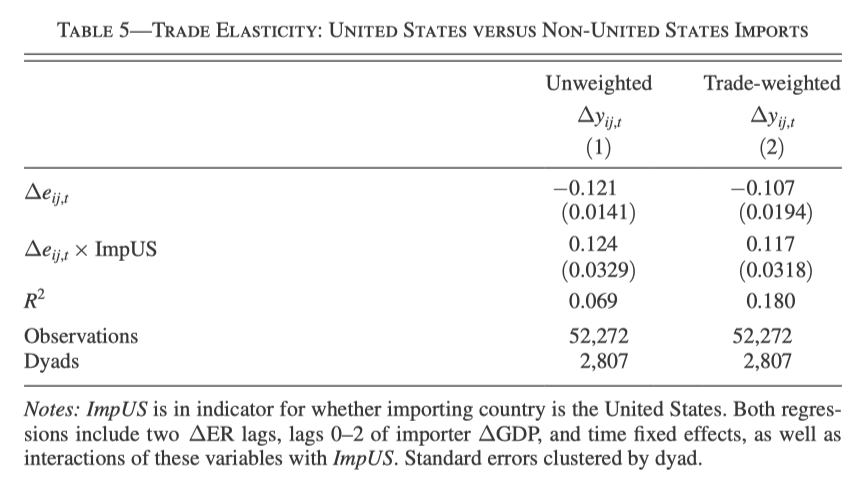
\includegraphics[width=11cm]{Table5.png}
    \end{figure}
\end{frame}
\subsection{Effect of US Dollar on Rest-of-World Trade and Inflation}
\begin{frame}{Effect of US Dollar on Rest-of-World Trade and Inflation}
    \begin{itemize}
        \item The last implication is about the dollar's impact on trade volume among countries in the rest of the world.
        \item \emph{When all countries’ currencies uniformly depreciate relative to the dollar, it should lead to a decline in trade between the rest of the world (i.e., excluding the United States).}
\end{itemize}
\end{frame}

\begin{frame}{Effect of US Dollar on Rest-of-World Trade and Inflation}
\begin{itemize}
    \item Panel regression function
        \begin{equation*}
            \begin{aligned}
                \Delta y_{i j, t}= &\sum_{k=0}^{2}\left(\beta_{k}+\eta_{k}\left(1-S_{j}-S_{j}^{euro}\right)\right) \Delta e_{i j, t-k}\\ 
                &+\sum_{k=0}^{2}\left(\beta_{k}^{\$}+\eta_{k}^{\$} S_{j}\right) \Delta e_{\$ j, t-k}\\
                &+\sum_{k=0}^{2}\left(\beta_{k}^{euro}+\eta_{k}^{euro} S_{j}^{euro}\right) \Delta e_{euro j, t-k} +\lambda_{i j}+\theta^{\prime} X_{i j, t}+\varepsilon_{i j, t}
            \end{aligned}
        \end{equation*}
    \item $S_j$ and $S_j^{euro}$ are the importer's country-level dollar and euro invoicing shares.
    \item Notice that to measure the effect of dollar appreciation against all other currencies, the time fixed effects are not controlled; several proxies for the global business cycle are controlled.
    \end{itemize}
\end{frame}
\begin{frame}{Effect of US Dollar on Rest-of-World Trade and Inflation}
    \begin{figure}[htp]
        \centering
        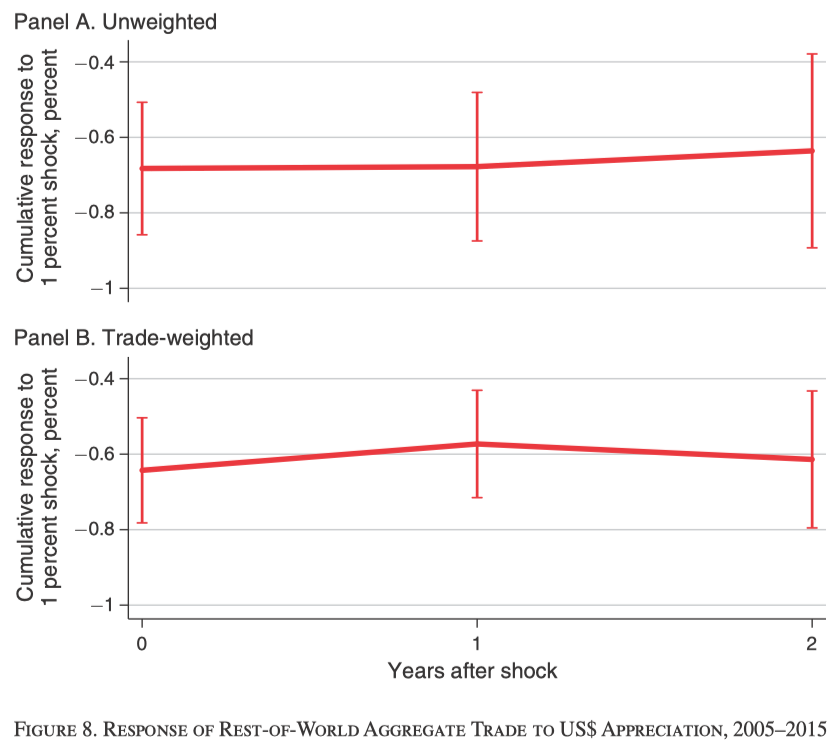
\includegraphics[width=9cm]{Figure8.png}
    \end{figure}
\end{frame}
\subsection{Calibration with Colombian Firm-level Data}
\begin{frame}{Calibration with Colombian Firm-level Data}
    \begin{itemize}
        \item The authors then calibrate their model using the firm-level customs data on exports and imports for a small open economy, Colombia.
        \item They use the noncommodity terms-of-trade and only focus on manufactured goods.
    \end{itemize}
\end{frame}
\begin{frame}{Calibration with Colombian Firm-level Data}
    \begin{figure}[htp]
        \centering
        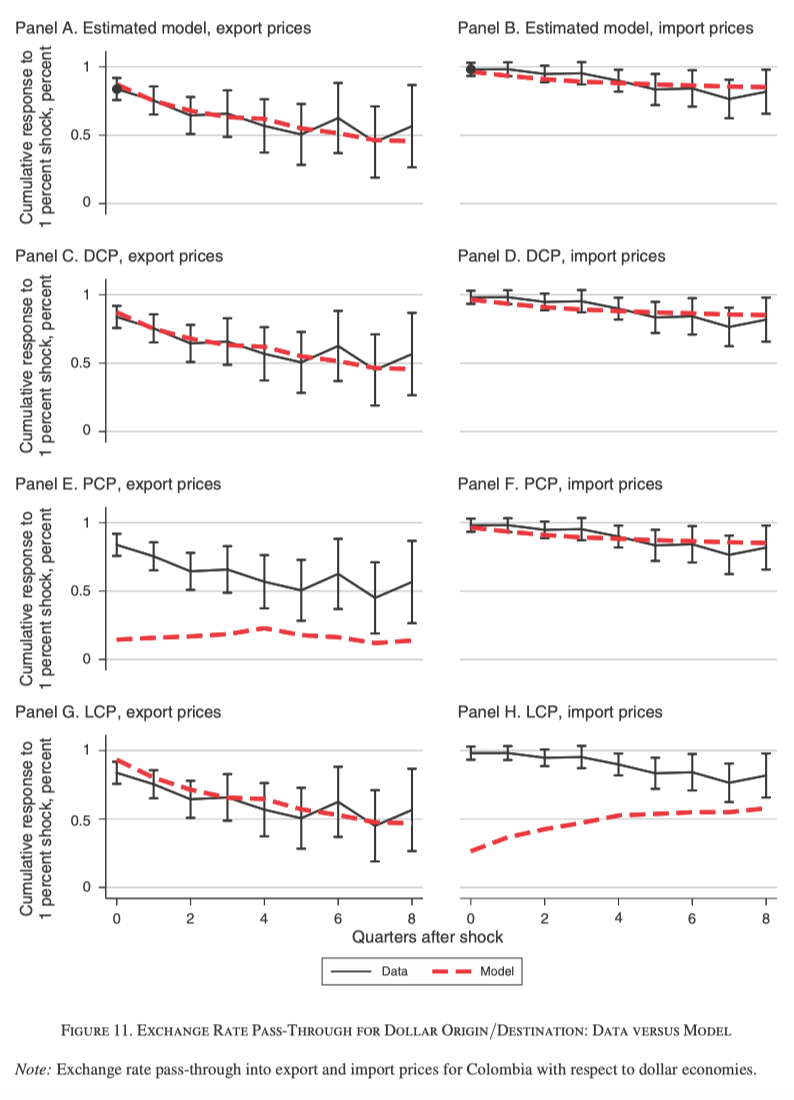
\includegraphics[width=5cm]{Figure11.png}
    \end{figure}
\end{frame}
\begin{frame}{Calibration with Colombian Firm-level Data}
    \begin{figure}[htp]
        \centering
        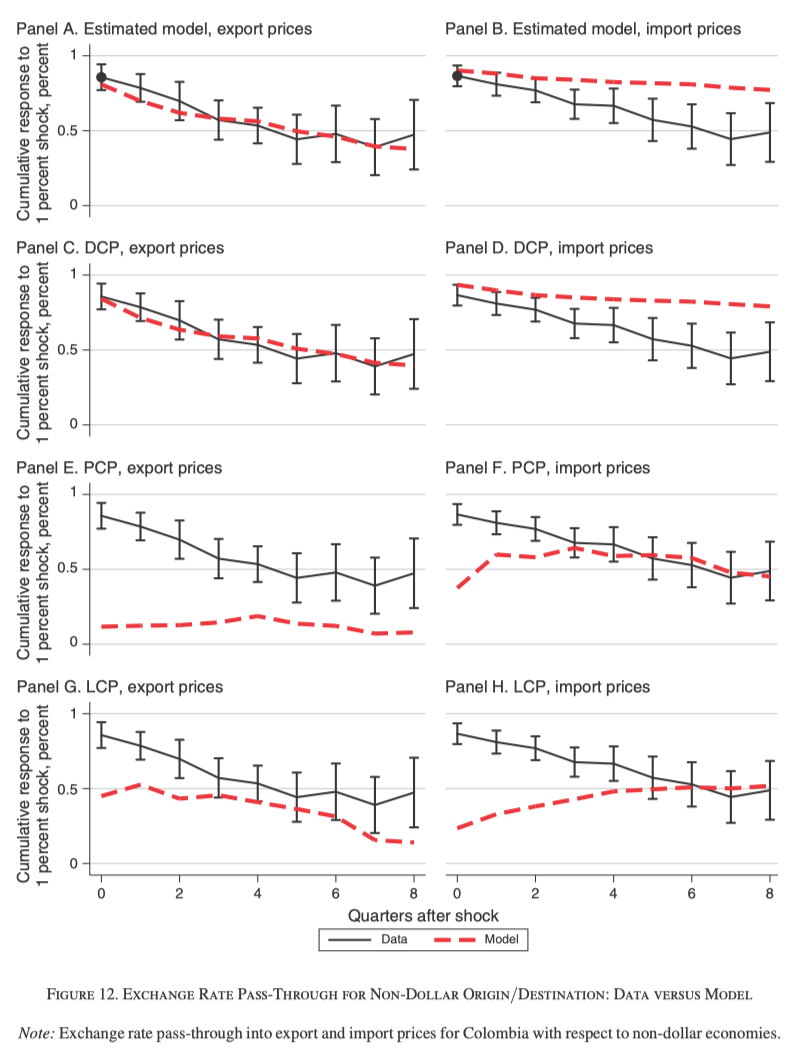
\includegraphics[width=5cm]{Figure12.png}
    \end{figure}
\end{frame}
\begin{frame}{Calibration with Colombian Firm-level Data}
    \begin{figure}[htp]
        \centering
        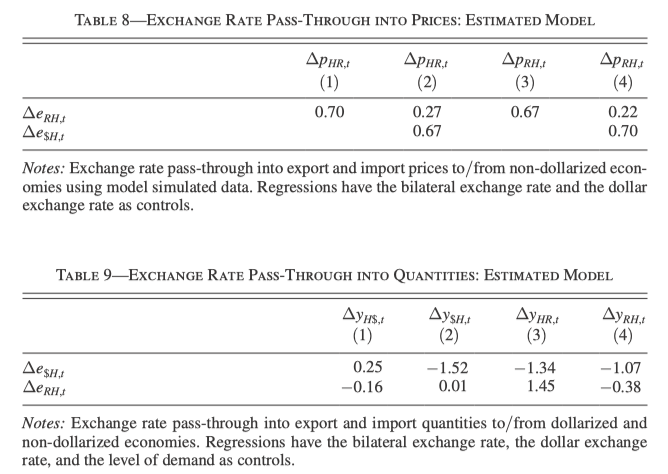
\includegraphics[width=9cm]{Table8.png}
    \end{figure}
\end{frame}
\section{Counter-evidence against DCP}
\begin{frame}{Counter-evidence against DCP}
\begin{itemize}
    \item Sarsenbayev and Gagnon (2021) counters the DCP hypothesis using the substantial uniform dollar appreciation of 2014-15 as a natural experiment.
    \item Only 2 out of 22 economies they examined experienced an increase in export prices, while the rest followed domestic prices or a trade-weighted average of prices in foreign currencies.
    \item They further categorized different economies into different currency paradigms based on the pattern of their export price movements.
\end{itemize}
\end{frame}
\begin{frame}{Counter-evidence against DCP}
    \begin{figure}[htp]
        \centering
        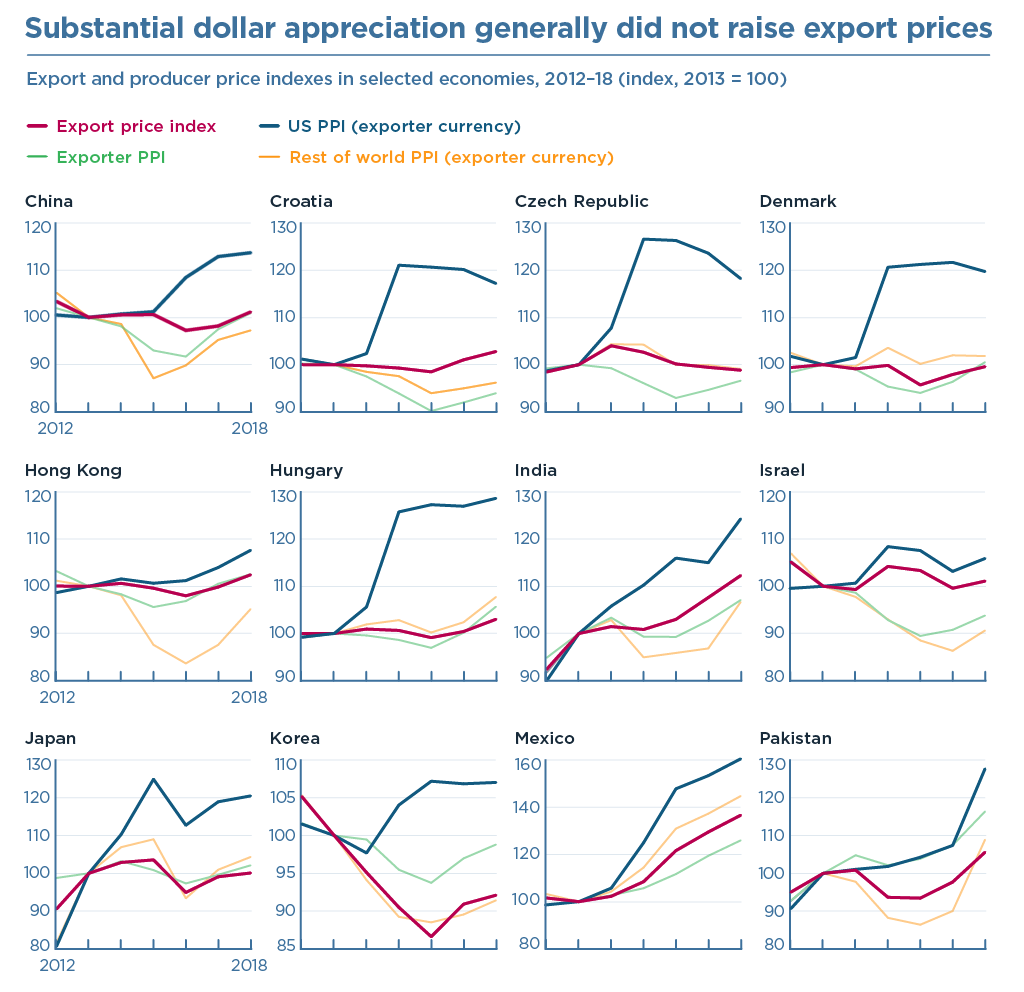
\includegraphics[width=7.5cm]{22countries.png}
    \end{figure}
\end{frame}
\begin{frame}{Counter-evidence against DCP}
    \begin{figure}[htp]
        \centering
        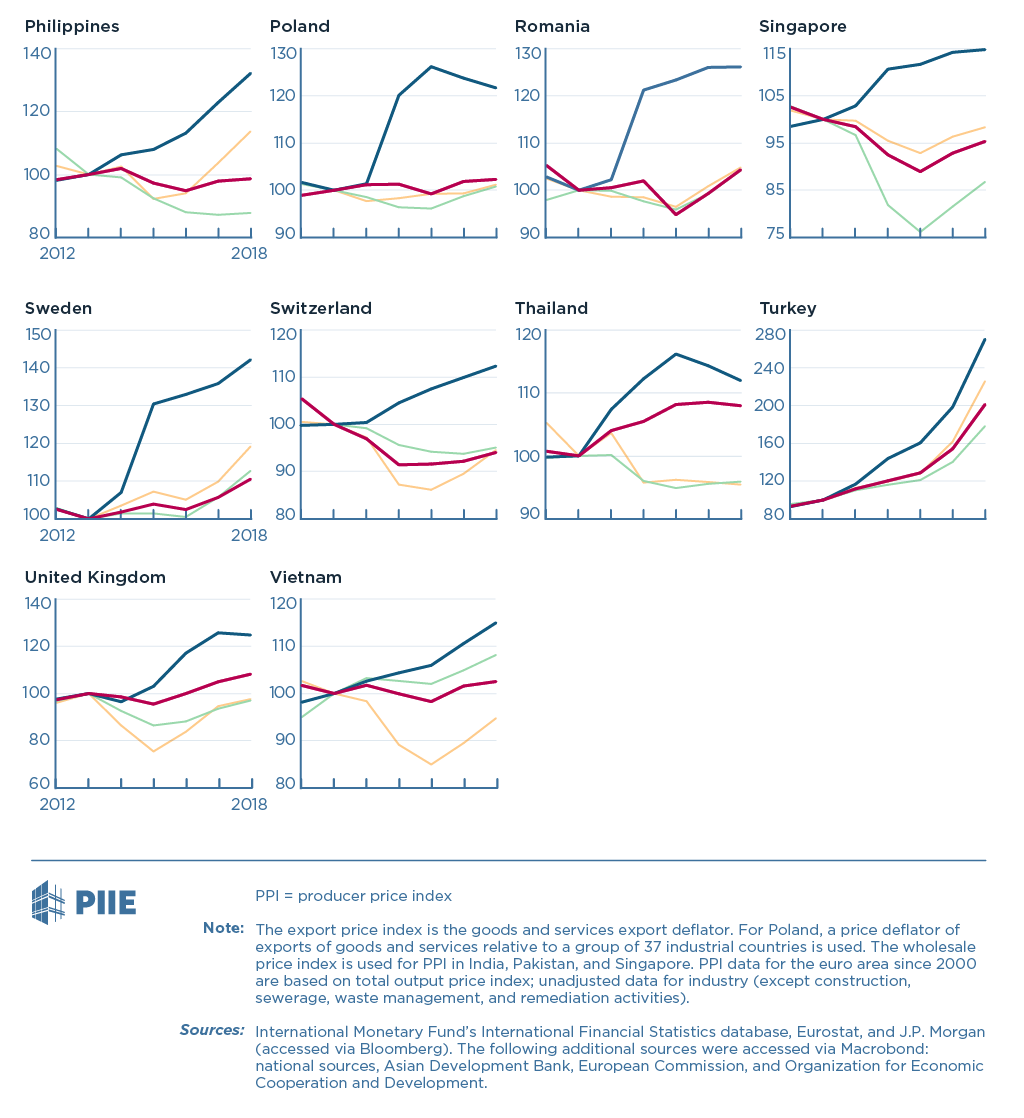
\includegraphics[width=7.5cm]{22countries copy.png}
    \end{figure}
\end{frame}
\begin{frame}{Counter-evidence against DCP}
    \begin{figure}[htp]
        \centering
        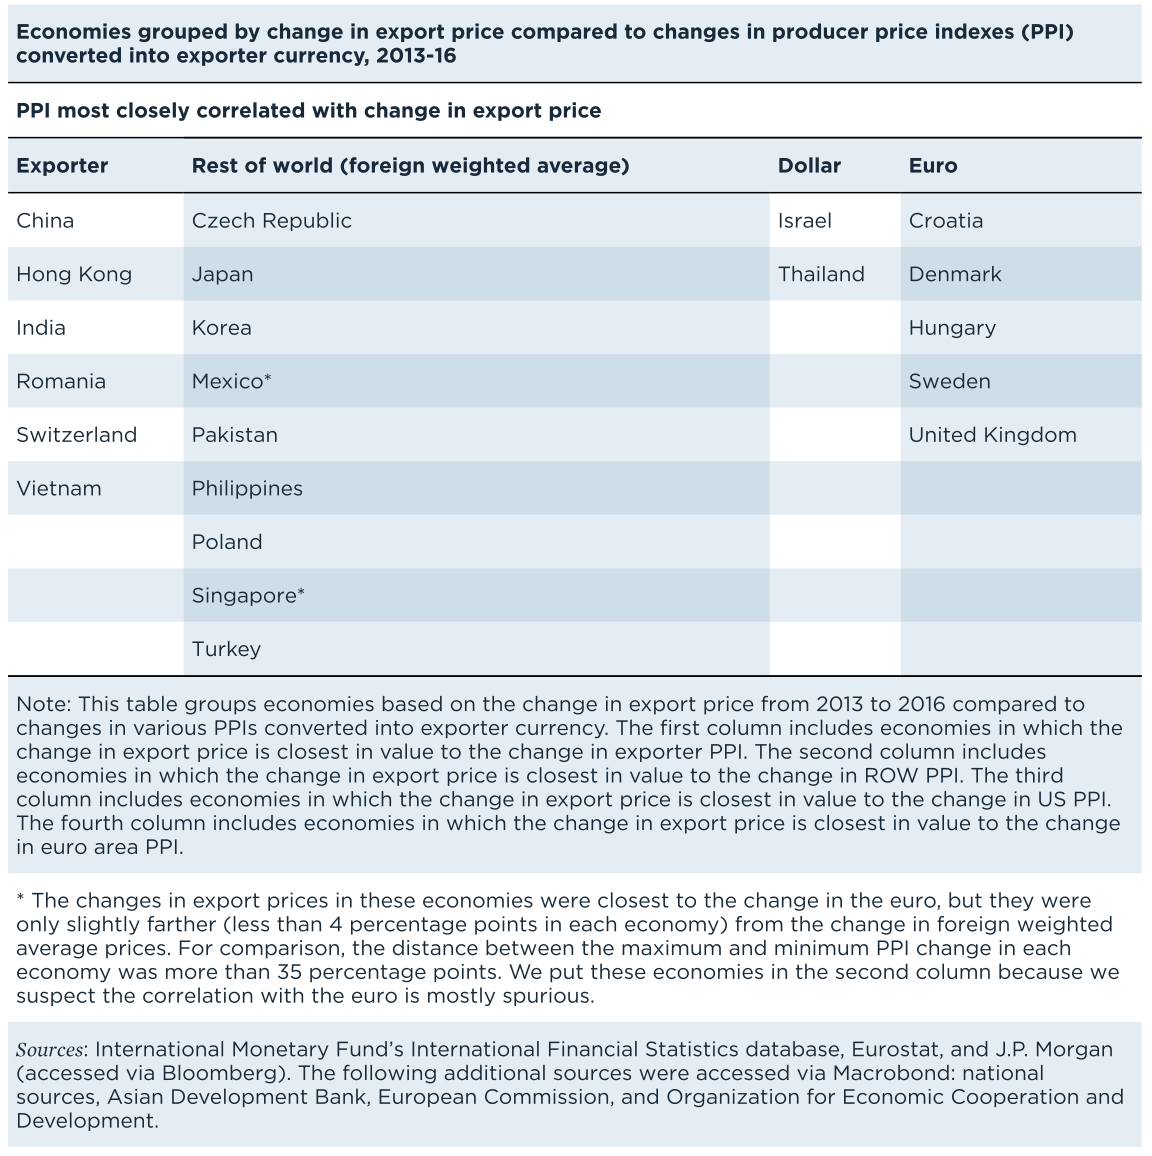
\includegraphics[width=7.5cm]{Group.png}
    \end{figure}
\end{frame}
\section{Closing Comments}
\begin{frame}{Closing Comments}
\begin{itemize}
    \item If DCP is the case, then the rest of the world outside the country that issues the dominant-currency is unable to influence the relation between export and import prices with their monetary policies.
    \item Recall that the IRF analysis showed that the inflation-output trade-off in response to a monetary policy shock for a small open economy worsens under DCP relative to PCP.
    \item This relates to the broader discussion of optimal monetary policy in open economy and the trilemma in international finance.
\end{itemize}
    
\end{frame}
\end{document}
